%----------------------------------------------------------------------------------------
% PACKAGES AND OTHER DOCUMENT CONFIGURATIONS
% WARNING: Don't mess with any of the following unless you know what you are doing.
%----------------------------------------------------------------------------------------
\documentclass[english,12pt,a4paper,openany]{book}
\usepackage{datetime}
\usepackage{tabularx}
\usepackage{makecell}
\usepackage{eurosym}
\usepackage{pbox}
\usepackage[utf8]{inputenc}
\usepackage[T1]{fontenc}
\usepackage[english]{babel}
\usepackage{amsmath}
\usepackage{amsfonts}
\usepackage{fancyhdr}
\usepackage{amssymb}
\usepackage[dvipsnames]{xcolor}
\usepackage{mdframed}
\usepackage{multirow}
\usepackage{multicol} 
\usepackage{tikz}
\usepackage{graphicx}
\usepackage[absolute]{textpos} 
\usepackage{colortbl}
\usepackage{array}
\usepackage{geometry}
\usepackage{hyperref}
\pagestyle{fancy}
\renewcommand\headrulewidth{1pt}
\usepackage{float}
\usepackage{tcolorbox}
\usepackage{accsupp}

\newcommand{\copyable}[1]{%
    \BeginAccSupp{%
        method=escape,
        ActualText={#1}
    }%
    #1%
    \EndAccSupp{}%
}

%------------------------------------------------------------------------------------------------------
%	The following are the RGB values for the official ATU colours.
%------------------------------------------------------------------------------------------------------	
\definecolor{ATUGreen}{RGB}{0, 91, 94}
\definecolor{ATULightGreen}{RGB}{172, 245, 189}
\definecolor{ATUNavy}{RGB}{0, 26, 121}
\definecolor{ATUOrange}{RGB}{255, 121, 30}
\definecolor{ATUPurple}{RGB}{77, 8, 87}
\definecolor{ATUSand}{RGB}{255, 232, 212}
\definecolor{ATUTeal}{RGB}{123, 185, 203}
\definecolor{ATUWarmGrey}{RGB}{200, 190, 191}
\definecolor{ATUYellow}{RGB}{248, 255, 142}



%------------------------------------------------------------------------------------------------------
%	******* CHANGE THE FOLLOWING VARIABLES
%------------------------------------------------------------------------------------------------------	

\newcommand{\reportauthor}{Katelyn Graham} % Change to your name
\newcommand{\projecttitle}{FILE A WHILE}
\newcommand{\reporttype}{Minor Dissertation} %Report  type (Project Plan / Final Report)
\newcommand{\supervisorname}{Joseph Corr} %Report  type (Project Plan / Final Report)
\newdateformat{monthyeardate}{\monthname[\THEMONTH], \THEYEAR}





%------------------------------------------------------------------------------------------------------	
% WARNING: Don't mess with any of the following unless you know what you are doing.
%------------------------------------------------------------------------------------------------------	
\pagestyle{fancy}
\fancyhf{}
\fancyhead[R]{\textcolor{ATUGreen}{\reportauthor}}
\fancyhead[L]{\textcolor{ATUGreen}{\projecttitle}}
\fancyfoot[L]{\textcolor{ATUGreen}{Atlantic Technological University (ATU), Galway.}}
\fancyfoot[R]{\thepage}

\begin{document}
\begin{titlepage}

\newgeometry{left=6cm,bottom=2cm, top=1cm, right=1cm}

\tikz[remember picture,overlay] \node[opacity=1,inner sep=0pt] at (2.2mm,-165mm){
\includegraphics{images/leftbar.png}}; % Fond changeable 

\fontfamily{fvs}\fontseries{m}\selectfont
\color{white}

\begin{picture}(0,0)
\put(-110,-743){\rotatebox{90}{\Huge{B.Sc. (Hons) in Software Development}}}
\end{picture}
 
\vspace{-10mm} 

\flushright 
\includegraphics[width=100mm]{images/atu-logo-green.png} 

\flushright
\vspace{10mm}
\textcolor{ATUGreen}{
\fontfamily{cmss}\fontseries{m}\fontsize{22}{26}\selectfont
\projecttitle
}
\normalsize
\color{black}

\vspace{1.5cm}
\normalsize
\textbf{By \\ \textcolor{ATUGreen}{\reportauthor}}\\ %Dr. John Healy
\vspace{15mm}
\textbf{for \\  \supervisorname}\\
\vspace{15mm}
{\scshape \today} \\[0.3\baselineskip]
\vspace{75mm}
\Large {\textcolor{ATUGreen}{\textbf{{\reporttype}}}} \\
\bigskip
\normalsize
\textbf{Department of Computer Science \& Applied Physics,\\School of Science \& Computing,\\Atlantic Technological University (ATU), Galway.}\\
\end{titlepage}
\newpage
\tableofcontents
\listoffigures
\pagenumbering{arabic} 

%----------------------------------------------------------------------------------------
%	   ******* CHANGE the Chapters if necessary. Each chapter is encapsulated inside 
%                 its own file. The chapters below are based on the guidelines 
%                 given in the lecture.
%----------------------------------------------------------------------------------------
\chapter{Introduction}	

In today’s digital age, file management and organisation are critical aspects of productivity and efficiency. However, traditional paper-based filing systems are no longer sufficient to meet the demands in the modern world. Due to the ever-rising development of technology, there is a need for a more user-friendly and efficient way of organising digital invoices for small businesses.  This is where the filing system web application comes in. The title of this project is “File A While”. The objective of this project is to design and develop a web-based application that facilitates effortless storage of invoices for the end users by offering a user-friendly interface. 

\section{Overview} 

This chapter aims to provide the reader with a comprehensive understanding of the project’s background and its primary objectives. Chapter 2 will describe the methodology that was taken into consideration when approaching the project, including the various collaborative tools utilised by the developer. In Chapter 3 a conceptual level overview of the primary technologies used in this project will be presented. This sets the foundation for Chapter 4, which will be an in-depth discussion of the system design. Chapter 5 will discuss the system evaluation and reflect on the objectives that were outlined in the introduction. It will also address the system’s current limitations and potential for future development. The sequence of the chapters taken together will provide a full analysis of the project’s scope and implementation.

\section{Background and Scope} 

The filing system is an essential tool for individuals and organisations to store and manage information effectively. With the increasing reliance on digital storage, there is a growing need for efficient and user-friendly filing systems that can adapt to changing needs and take advantage of the new technologies available. In the context of this project, the present study aims to develop a filing system web application that utilises both frontend and backend technologies. The application in relation to this dissertation will be developed using React Native for the front end and Node.js for the backend. This dissertation will provide a comprehensive overview of the development process. It will highlight the challenges, solutions and outcomes of the project. By addressing key research questions related to the development process. 
\newline \newline
The development of web applications has seen rapid growth in recent years, with businesses and organisations turning to these applications to engage with customers and manage their operations. This trend has been driven by the increasing availability and accessibility of mobile devices and internet connectivity. 
\newline \newline
With the growing demand for web applications, there is a need for developers to create applications that are user-friendly, scalable and secure. The development of a Filing System Management Application requires a deep understanding of the principles of frontend and backend development, as well as the ability to design a system that is intuitive and meets the needs of users. In this context, the present study aims to develop a filing system web application that leverages the strengths of React Native and Express.js/Node.js, providing users with an efficient and user-friendly platform to manage their information.
\newline \newline
The traditional methods of filing and managing information, such as physical paper-based systems, are becoming outdated with the rise of digitalization. However, while digital filing systems offer several advantages over their physical counterparts, they can be complicated and difficult to manage, particularly when dealing with large amounts of data. Existing filing systems may be slow, outdated or insecure, creating inefficiencies and security risks for organisations and individuals alike. Additionally, many existing filing systems do not provide a user-friendly interface, making it difficult for users to access and manage their information. In response to these challenges, the present study aims to develop a filing system web application that addresses the shortcomings of existing systems, providing users with a platform that is efficient, user-friendly and secure.
\newline \newline
The purpose of this study is to develop a filing system web application that utilises React Native for the frontend and Express.js / Node.js for the backend. The application will be designed to provide users with an intuitive and efficient platform to manage their information. The study will explore the various design considerations and challenges associated with developing such an application, including user interface design, database management, security and scalability. The study aims to answer several research questions related to the development, such as: What are the key design considerations for developing a user-friendly and efficient filing system web application? What are the best practices for integrating frontend and backend technologies to create a cohesive application? How can security risks be mitigated when developing a web application that deals with sensitive information? By answering these questions, the study aims to contribute to the growing body of knowledge on effective web application development and provide practical insights for developers seeking to create user-friendly and secure filing system applications.

\section{Objectives} 

With the background provided above, the below will outline the main objectives set for this project and personal objectives set out by the developer.
\subsection{Project}
\begin{itemize}
    \item To develop a mobile application which enables small businesses to efficiently process their invoice management by providing a convenient digital platform to organise and file invoices with ease.
    \item Develop an application that will make the management of invoices easier for small enterprises by providing a digital platform to organise and store their invoices. 
    \item Eliminate the need for excessive paper documentation and simplify the process of tracking invoices.
    \item Develop a fully operational web application with minimal defects 
\end{itemize}

\subsection{Personal}
    \begin{itemize}
        \item Learn how to use React Native effectively and feel confident applying it
        \item Increase knowledge of JavaScript programming language
        \item Create a minimally flawed application that is fully functioning and user-friendly
        \item Create an application that helps small businesses to manage and store their invoices online, eliminating the need for endless paperwork
    \end{itemize}

\section{Work Breakdown}
This section will give an overview of the work carried out in this project

\subsection{Project} 
\begin{enumerate}
    \item Research conducted throughout the project
    \item Planning of the applications using wire frames, Jira, etc.
    \item Backend
        \begin{itemize}
            \item Create a basic Node.js App
            \item Set up web server
            \item Configure MySQL database and Sequelize
            \item Define the Sequelize Model
            \item Create the controller (CRUD objects)
            \item Define Routes
            \item Test the API
        \end{itemize}
    \item Frontend
        \begin{itemize}
            \item Initialise an Expo app
            \item Splash Screen
            \item Drawer Navigation
            \item Log In Screen
            \item Registration Screen
            \item Home Screen
            \item Setting Screen
            \item Screen to View All Invoices
            \item Add Invoice Screen
            \item Individual Invoice Summary Screen
        \end{itemize}
    \item Integrate and Test
    \item GitHub
\end{enumerate}
\subsection{Dissertation}
\begin{enumerate}
    \item Research
    \item Abstract
    \item Introduction
    \item Methodology
    \item Technology Review
    \item System Design
    \item System Evaluation
    \item Conclusion
\end{enumerate}

\section{Source Code}
This section contains the link to the relevant GitHub repository for this project. 

\subsection{Applied Project}

The below URL directs to the primary Git repository used for this project’s development. It contains all the code from the frontend and backend.

\href{https://github.com/katelyngraham1/Final_Year_Project}{https://github.com/katelyngraham1/Final\textunderscore Year\textunderscore Project} 


\subsection{Dissertation} 
This URL points to the source control for this latex document. Readers can refer to the above repository for more detail on the project’s implementation.

\href{https://github.com/katelyngraham1/Final_Year_Dissertation}
{https://github.com/katelyngraham1/Final\textunderscore Year\textunderscore Dissertation}



\subsection{Video Demo}
This URL points to the demo video. This video goes through the application and explains how to use the it.

\href{https://youtu.be/oJY_FlK4dSM}
{https://youtu.be/oJY\textunderscore FlK4dSM}




\chapter{Methodology}
This chapter discusses methodologies used throughout the project, such as the software development methodology, testing and project management used within the project.
\newline 

\section{Software Development}
The software development process was broken into the following main phases:
\begin{itemize}
    \item High Level Design – the main focus of this phase of the development was to produce an overall architecture for the system, separating the system out into its main elements and defining the clear interfaces between them. As part of this initial phase a set of screen mock-ups and associated supporting API end points were mapped out, and the initial database model design was scoped out.
    \item Low Level Design and Coding – for this phase I was able to build on the high-level design, finalising the specific design details and then code/ implement both the Frontend App and the backend server. The development of the also backend included the creation of the application database model using MySQL.
    \item Integration Testing - the main focus of this phase was to combine together the various elements and to perform a comprehensive suite of tests against the system to verify that all aspects functioned as expected.
\end{itemize}
As mentioned, the application can be broken into two sections, the frontend and the backend. As part of the coding phase the backend element of the system was developed and tested first before starting on the front end, which made it a lot easier to identify issues and fix them as they arose. 

\subsection{Backend}
To develop the backend for this project, a RESTful API was built using Node.js, Express, Sequelize and MySQL. The purpose of the backend is the manage the data for the project. This involves both the registration and login of users, and then creating, reading, updating and deleting (CRUD) data in a database. 
The development process for the backend was followed using the steps that were outlined in a tutorial found on a website. \cite{bezkoder} This tutorial allowed for a structured approach when building the backend. The tutorial covered everything from setting up the development environment to deploying the application on a server. 
\newline \newline
Before starting on the coding, the required software and tools were installed on the development machine. This included Node.js, the server-side JavaScript runtime, and the Express framework which is a fast and minimalist web framework for Node.js that is used to build web applications. MySQL, which is the database management system, was installed using the installation instructions given by the website. \cite{mySQLinstall} Once the necessary software and tools were installed, the tutorial was followed step-by-step to create the necessary files and directories for the backend application. The tutorial offered a basic structure for the application, which was then modified and expanded to meet the specific requirements for this project as shown in Figure \ref{fig:backendDirectory}
\begin{center}
    \begin{figure}[h!]
        \centering
        \label{fig:backendDirectory}
        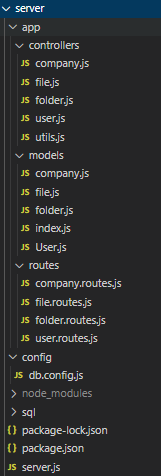
\includegraphics[height=0.40\textheight]{images/backendDirectory.png}
        \caption{Backend Directory}
    \end{figure}
\end{center}
The next step was to create a connection from the backend to the MySQL database. In order to do this, the connection information, including the database name, username and password, had to be defined in a configuration file, i.e. db.config.js. The connection to the database was then made using the Node.js MySQL driver. After the connection was made, a SQL script that specified the tables and their columns was run to create the database structure. 
\newline \newline
Following that, the API routes were then built. To be able to connect with the data in the database, a set of HTTP endpoints needed to be created. The routes were set up using the Express framework, which also dealt with HTTP requests and responses. The RESTful design of the API routes ensures that they follow a set pattern for record creation, reading, updating and deleting. To implement the CRUD operations, the Node.js MySQL driver was used to execute SQL statements that interacted with the database. The parameters given in the HTTP requests were used to generate the SQL statements on their own. This made it possible for the API to manage a variety of requests and provide the right information in response. 
\newline \newline
To ensure that the backend is reliable and well secured, various measure were taken. For example, input validation was implemented to make sure that API would only accept accurate data. Error handling was also put into place to give clients a clear error message when errors occurred. Lastly, authentication was implemented to further limit access to the API to authorised users.
Node.js was used to control the data flow across the application and speed up the request-response process. The middleware functions were used to carry out tasks like parsing incoming requests, recording requests and responses, and managing problems.
\newline \newline
Overall, the development of the backend by using the tutorial \cite{bezkoder} was a critical component of this project.  The tutorial provided a solid foundation that the developer then customized to meet the specific needs that the project entailed. The resulting RESTful API provides a secure and reliable backend for the managing of the project data.


\subsection{Frontend}
In order to develop the frontend for this project, the Expo framework was chosen due to its ease of use and efficiency in developing cross-platform applications. To set Expo up the steps outlined in the following Expo documentation was followed, \cite{buildRNscreen}. This ensured that all necessary software and tools were installed on the development machine. After the necessary software was installed, a new Expo project was created using the command-line interface that Expo provides. This is the client folder in the project. The command used to do this is \textbf{\emph{‘expo init’}} . A straightforward, simple test screen was designed by the developer to verify that the expo project was functioning.
\newline \newline
The next step was to install the React Native CLI. This involved adding React Native to the project using the command line interface and the command \textbf{\emph{‘react-native init’}}. The text editor of choice was Visual Studio Code. From the command line, this editor can be open by using the command \textbf{\emph{'code .'}} .
\newline \newline
The React Native framework was selected for its cross-platform compatibility and efficient developer process. To start on the features for the app, the developer decided to start by implementing the  Log in and Signup screens \cite{login&reg}. For these navigators were needed in the project and to use them there was a few dependencies that needed installing. Here are the sets needed for this:
\newline \newline
\begin{itemize}
    \item Change into the correct directory: 
        \begin{center}
            \begin{tcolorbox} [colback=gray!20!white,colframe=gray!50!black,width=0.5\linewidth]
                \centering\copyable{cd (Project Name) }
            \end{tcolorbox}
        \end{center}
    \item React Navigation: 
        \begin{center}
            \begin{tcolorbox} [colback=gray!20!white,colframe=gray!50!black,width=0.7\linewidth]
                \centering\copyable{‘npm install @react-navigation/native –save’}
            \end{tcolorbox}
        \end{center}
    \item Other Supporting libraries for react-navigation: 
        \begin{center}
            \begin{tcolorbox} [colback=gray!20!white,colframe=gray!50!black]
                \centering\copyable{‘npm install react-native-reanimated react-native-gesture-handler react-native-screens react-native-safe-area-context @react-native-community/masked-view –save’}
            \end{tcolorbox}
        \end{center} 
    \item Drawer Navigation: 
        \begin{center}
            \begin{tcolorbox} [colback=gray!20!white,colframe=gray!50!black,width=0.7\linewidth]
                \centering\copyable{‘npm install @react-navigation/drawer –save’}
            \end{tcolorbox}
        \end{center}
    \item Stack Navigation: 
        \begin{center}
            \begin{tcolorbox} [colback=gray!20!white,colframe=gray!50!black,width=0.7\linewidth]
                \centering\copyable{‘npm install @react-navigation/stack –save’}
            \end{tcolorbox}
        \end{center} 
    \item Install async-storage to use AsyncStorage: 
    \begin{center}
            \begin{tcolorbox} [colback=gray!20!white,colframe=gray!50!black]
                \centering\copyable{‘npm install --save @react-native-community/async-storage’}
            \end{tcolorbox}
        \end{center}
\end{itemize}
Once all dependencies where installed, React Native components were used to build the login and registration screens. The form inputs needed in these screens were managed using the \emph{‘TextInput’} component and the \emph{‘Button’} component was used for the log in and register buttons. Using the \emph{‘StyleSheet’} component the developer made the screens look appealing to use. Once this was done the next step was to create a new navigation stack by importing the \emph{‘createStackNavigation’} from \emph{@react-navigation/stack}. By using this function, it can take an object as its parameter that defines the screens and their navigation options. In this case, the two screens defined were LoginScreen and RegisterScreen. 
\newline \newline
Now the options for each screen could be defined. This covers choices such as the screen title, header design and navigational style. The screens chosen for this were the HomeScreen and the SettingsScreen. By designing basic screens the developer was then able to test if the navigation system was properly working.







\section{Project Management}
 
This section will describe the various development tools that were used throughout the period of the project's development.

\subsection{Microsoft Teams}

The Microsoft Teams application was frequently used for virtual meetings with the supervisor. In these meetings the project process from the previous week, the plan for the following week and feedback from the supervisor was discussed. Meetings with the supervisor were initially all in person but with changing time schedules they were brought online to facilitate both parties. Microsoft Teams was very beneficial for meetings as it was easy to share screens and other documents with the supervisor. There was not much difference between in person ad online meetings when using Microsoft Teams. This application allowed for a weekly scheduled meeting that was added to both developer and supervisors’ calendars. It also sent reminders 30 minutes before the meeting to both parties. However, having good internet access was a necessary requirement to be able to use the application. 

\subsection{Google Slides}

To plan the design of the app, Google slides was used to draw up wireframes. This let the user create diagrams, schemas and map out the layout for the application. Google Slides is a collaborative tool, so it was easy to share these slides with the supervisor to be able to get feedback. These diagrams are later seen in Figure \ref{image:wireframe}

\subsection{Jira}
Jira was used to implement a project management methodology. This was based on 2-week sprints. This software provided the ability to add issues to sprints at any time of the development. This meant that the planning was flexible and was able to have adjustments made when needed. Also, any tasks that were incomplete in the previous sprint was automatically carried over to the following sprint. This ensured that the project was always moving forward, and progress was not lost as the task could be complete in the next sprint. By using Jira software it meant there was a structured approach to the management of the project. It allowed for the developer to have a clear visualisation of what had to be done and allowed for easy tracking of the progress that had been made already. By being able to edit sprints and carry over unfinished tasks it made it simple to manage the project and ensured that all tasks were complete within the planned timeframe, as some weeks the developer could get more work done than others. 
\newline \newline
Additionally, with the use of epics, the user was able to break larger tasks into smaller tasks. For example when creating the Authentication part of the project, the developer could break it down into log in, log out and register. This created a high level of organisation and made it less daunting for the developer when they went to implement a large task.




\addtocontents{toc}{\protect\newpage}
\chapter{Technology Review}
One of the most critical aspects of software development is choosing the right technology stack. This chapter will discuss the technology stack used for the development of this mobile application. Jira was used to track and manage the project's progress from start to finish. The main project technologies used to undergo this project can be split into two categories: frontend and backend. The former consists of the React Native application. Expo was used to simplify the testing and deployment for the frontend of this project. The latter consists of a Node.js Rest API with Express, Sequelize and MySQL. Postman was used to test the backend before working on the front end.


\section{Jira}
Jira is a project management tool developed by Atlassian\cite{atlassian}. It is designed to help teams plan, track and manage projects efficiently. It is becoming more common for teams in the software development industry to use an agile development methodology, with many teams adopting the use of sprints to organise their work. Sprint planning helps break down complex projects into smaller, more manageable tasks, allowing teams to focus on specific goals and deliverables. This enables better project planning and more accurate estimation of the time and resources required to complete the project.  Sprints promote collaboration and communication between team members. It can help avoid isolation or miscommunication and ensures that everyone is on the same page, leading to better results and higher quality output. Users can create and assign user stories to team members, set deadlines and track progress through the sprint. Additionally, Jira provides a range of project management tools, including time tracking, reporting and custom workflows, to help teams stay organised and focused.
\newline \newline
At first, Jira’s interface can be a bit overwhelming for a new user, but once familiarised with its layout, it is relatively easy to use. The platform is highly customizable, allowing the user to tailor the interface to their specific needs. However, the customization options can also make the platform somewhat complex and time consuming to set up. Jira integrates with a range of other tools commonly used in software development, e.g. Git. This integration allows teams to easily share information and collaborate across different platforms, making it easier to manage complex projects. 
Jira is a popular asset due to its scalability. It can be used by teams of all sizes, from as small as an individual project to large enterprises. 

\section{React Native}

React Native is a popular open-source mobile application development framework. \cite{danielsson2016react}It enables developers to build native mobile apps using JavaScript and React, a popular web development framework. React Native is built on top of React, which allows developers to use a declarative programming model to describe the desired user interface of an application. This approach can make it easier to build and maintain code and can also improve performance. 
\newline \newline
One of the key benefits of React Native is that it enables developers to build mobile apps for both IOS and Android platforms. \cite{RNbenefit} This can save time and effort compared to building separate codebases for each platform and can also make it easier to maintain and update code. Due to React Native using a declarative programming model, it allows developers to describe the desired user interface, rather than how to achieve it. This approach can make it easier to develop and maintain code, as well as improve the performance of the application. 
\newline \newline
React Native also offers several other benefits. Cross platform compatibility is one of the core features of React Native, which allows developers to write a single codebase that can run on both IOS and Android devices. This is achieved by using a set of core components and APIs that abstract away the platform specific differences and allow the app to run consistently across both platforms. Some of the key features and benefits of cross platform compatibility are:
\begin{itemize}
    \item Single codebase: With React Native, developers can write a single codebase that can be used to build apps for both IOS and Android devices, which can save time and effort compared to developing separate apps for each platform.
    \item Native performance: Despite the use of a single codebase, React Native apps are still able to deliver native performance and user experience on both platforms. This is achieved by using platform specific code where necessary, such as handling UI rendering and interactions
    \item Faster development cycle: React Native can also help to speed up the development cycle by allowing for faster iterations and testing. Since changes made to the codebase are immediately reflected on both platforms, developers can quickly test and iterate on their app’s features and user experience.
\end{itemize}	
Another key benefit of React Native is its large and active developer community. Ways in which a large developer community can be beneficial for React Native are as follows: 
\begin{itemize}
    \item Access to support and resources: With a large developer community, there are many resources available for developers to learn and troubleshoot issues with React Native. This includes online forums, blogs, tutorials and documentation which can help speed up the development process and provide solutions to common problems.
    \item Open-source contributions: React Native is an open-source project. This means that developers  can contribute to the development of the framework and its associated tools. With a large developer community, there are many opportunities for developers to contribute code, bug fixes and new features, which can help to improve the overall quality and functionality of React Native.
    \item Career opportunities: Finally, a large developer community can provide career opportunities for developers who specialise in React Native. With a growing demand for mobile app development, particularly for cross-platform apps, developers with React Native expertise are in high demand, and can benefit from a strong and supportive community.
\end{itemize}
Overall, the benefits of a large developer community in React Native are many and varied. With a large and active community, developers of the framework can leverage third-party libraries and tools, drive innovation and growth and benefit from career opportunities in the mobile app development industry.
\newline \newline
React Native provides a rich set of core components and APIs for developers to build mobile apps. However, there may be cases where developers need to add additional functionality or extend the capabilities of their app beyond what is provided in the core framework. In these cases, developers can turn to third-party modules or libraries that have been developed by the community. Third-party modules in React Native are typically published as NPM packages, which can be installed using the npm or yarn package manager. Once installed, these modules can be imported into React Native app like any other JavaScript module. There are many third-party modules available for React Native covering a wide range of use cases, from UI components and animations to data storage and networking. Some popular third-party modules for React Native include:
\begin{itemize}
    \item React Navigation: This is a library that provides a flexible and extensible way to handle navigation and routing in React Native apps.
    \item React Native Elements: A UI toolkit that provides a set of customizable and easy to use UI component.
    \item Axios: A library that provides a simple and powerful way to make HTTP requests in React Native apps.
\end{itemize}
While third-party modules in React Native can provide valuable additional functionality, there are some limitations and challenges to consider when working with them.
\newline \newline
 It is important to consider the compatibility of the module with the version of React Native being used. Third-party modules may not always be compatible with the latest version of React Native or other modules that are already installed in your project. This can lead to issues such as crashes or unexpected behaviour. Some third-party modules may impact the performance of your app, either by increasing memory usage or slowing down the rendering of UI components. It’s important to carefully review the documentation, evaluate the performance impact and compatibility information for each module before installing it in your project and consider alternatives if necessary.
 \newline \newline
React Native has other limitations \cite{RNlimitation} such as access to native functionality. React Native provides access to many native device features, there may be some functionality that is not available, which can limit the scope of certain applications. An example of the limited access to native functionality can include the advanced camera features. React Native provides basic camera functionality but does not support more advanced features such as manual focus or manual exposure control. Although React Native provides a wide range of built in UI components, there may be some cases where developers need to create custom UI components that are not available in the framework. React Native also does not support all types of app extensions, such as keyboard extensions or SiriKit extensions on IOS.
\newline \newline
Another limitation with React Native is the learning curve that is associated with the framework. There are many similarities between both React and React Native as React Native is based on the React library web development, but although there are many similarities, there are some important differences between the two. A developer that is familiar with React may have to learn new concepts such as the differences between components and screen, as well as the structure of a typical React Native app, when starting to program with React Native. React Native has a rapid pace of development and is constantly introducing regular updates to the framework, which often brings new features and improvements, but these updates can also introduce problems such as breaking code or making developers update their existing code. This can then add additional time and effort for the developer to be able to stay up to date with the latest version of React Native and make sure there is compatibility with other third-party modules or libraries.
\newline \newline
In conclusion, React Native is a powerful and versatile mobile development framework that can enable developers to build native mobile apps with a single codebase. Its cross-platform compatibility, large developer community and other benefits make it an attractive option for building mobile apps. However its limitations with respect to access to third-party module compatibility, native functionality and learning curve should also be considered when evaluating its suitability for a particular project. Despite these limitations, many developers find that the benefits of React Native, outweigh the limitations. By investing time and effort in learning React Native and staying up to date with the latest updates and best practices, developers can effectively leverage the framework to build high quality mobile apps.
       
\section{Expo Go}

Expo Go is an open-source platform that allows developers to build, test and deploy native mobile applications using JavaScript and React Native. \cite{expoGo} Expo Go is popular with developers that want to make cross-platform apps that work with IOS, Android and the web.
\newline \newline
One of Expo Go’s main advantages is that it offers a set of tools that reduce the development process, this makes it both faster and more efficient. Hot reloading is a significant benefit when using Expo Go as it allows the developers to see the code changes instantly without having to restart and wait for the application to load up. Due to this function it can be helpful when testing and debugging apps. This often means the developer spends less time fixing problems, improving the overall performance of the app.
\newline \newline
Expo Go gives access to a variety of pre-built components and libraries that are easy to add into the application. By using this, developers are able to reduce the time in which it takes to create complicated applications with innovative features. Additionally, Expo Go offers a number of features that may be used to improve the functionality of the app. This includes push notifications, in app purchases and much more. Due to the services being fully integrated with the Expo platform, these services make it simple to update the apps functionality as needed.
\newline \newline
Expo Go is widely regarded as being a dependable and stable platform with decent support for both IOS and Android smartphones in terms of performance. Expo provides excellent support for new technologies such as augmented reality (AR) and virtual reality (VR). These new technologies can be combined with an app using the Expo AR and Expo VR libraries. 
\newline \newline
Another benefit of Expo Go is that it supports a shorter development process. This can be especially helpful for small teams and individual developers who might not have access to the tools and support that a bigger development team would have. This can lower expenses and increase productivity, enabling developers to concentrate on making high quality programs that satisfy their consumers expectations. 
\newline \newline
Although Expo Go is a reliable software, it does contain some limitations that developers should be aware of before starting to use it when undergoing a project. It does not offer the same level of customization and control as other platforms, which could be a disadvantage to more experienced developers who would need more freedom and control over their code. The pre-built components and libraries may not be suitable for some developer’s particular needs which may then prolong the development process and cost them time. A strong understanding and knowledge of JavaScript and React Native are needed when using Expo Go. If a developer is unfamiliar with these technologies, they could end up needing additional training or assistance in order to use the platform efficiently. 
\newline \newline
Overall, Expo Go is a strong and flexible platform that offers a variety of tools and services to assist developers in producing high quality mobile applications. \cite{expoWithRN} Similarly to React Native, it contains limitations that can make it hard for developers to use but the advantages weigh out the disadvantages as it is widely regarded as a dependable and effective option for programmers who want to build cross-platform applications that work on iOS, Android and the web.



\section{Node.js}
Node.js is an open-source, cross-platform runtime environment for JavaScript that helps developers to create scalable and high-performance applications. \cite{node} It is built on top of the Google V8 JavaScript engine and provides an event-driven, non-blocking I/O model, making it perfect for developing real-time applications. Node.js can make an effective backend tool for applications, especially when used alongside the Express web framework, Sequelize and MySQL database.
\newline \newline
Using Node.js has many advantages, \cite{nodePro&Cons} one of them being its ability to handle multiple concurrent requests. This is due to the server’s non-blocking I/O model, which allows it to handle many requests simultaneously without causing any other requests to be blocked. Node.js can effectively handle high traffic volumes and as a result of this there is very little lagging. Another benefit to using Node.js is that it has a large and active community that is always developing new modules and libraries, making it simpler for developers to create complex applications. Additionally, there are a lot of third-party packages for Node.js that are accessible through npm. This can speed up the development by offering pre-built functionality that can be used in most projects.
\newline \newline
It is easy to create a scalable and effective REST API that can handle multiple requests at the same time using Node.js. The Express framework offers a set of tools and features that make it simple to create routes middleware and handle errors, making it very well-suited to developing RESTful APIs. It is easy to manage data and relationships between tables when using Sequelize to work in an object-oriented way with a SQL database. With regards to a particular stack, using Node.js with Express, Sequelize and MySQL, it provides a solid and effective basis for building a backend. MySQL is a popular and reliable relational database. It offers quick and scalable data storage. Sequelize makes the process of working with MySQL a lot simpler. It provides an object-relational mapping layer which allows the developer to work with the database in an object-oriented way.
\newline \newline
Like most technologies Node.js has its limitations. Some of the limitations in which Node.js has is there is no built-in support for relational databases. Although it can work with MySQL using ORM libraries such as Sequelize, it doesn’t have any built-in support for when a developer is working directly with SQL databases. This means developers have no choice but to rely on third-party libraries and tools to work with SQL databases. There can also be issues with backward compatibility. As Node.js has a short enough release cycle, newer versions may not be able to work with older code.  
\newline \newline
Overall Node.js is a powerful tool when it comes to building a backend that can handle high traffic loads efficiently. It offers a scalable and reliable framework for building a RESTful API when used with Express, Sequelize and MySQL. Although it has some minor limitations, it has a large and active community that is always developing new modules and libraries, which makes it a lot easier for developers to build complex applications.



\section{Sequelize}
Sequelize is an Object-Relational Mapping (ORM) library for Node.js. \cite{sequel} It offers an easy way to work with relational databases like MySQL, SQLite and many more. It provides excellent support for database synchronisation, eager loading, association, transactions and database migration. This can help simplify the database management process. With Sequelize, developers can easily synchronise their database schema with their application models, load similar data in a single query, define complex relationships between models and manage database migration.
Sequelize also includes security features that can help prevent SQL injection attacks. This is a common enough attack for web applications. It provides built-in parameterised queries, making it more difficult for attackers to inject malicious code into SQL queries. Along with that, it works well with other popular Node.js libraries and frameworks, such as Express. This means that developers can easily integrate Sequelize into their already existing applications and use its powerful features without having to completely re-design their application.
However, Sequelize may not be the best choice for every project. First of all, it has a steep learning curve, especially for developers that are new to ORMs and/or are not familiar with JavaScript Promises. Also, while it provides a convenient way to work with databases, not all are suitable as they could be too complex or need highly customisable database interaction. In these cases, it may be necessary to write raw SQL queries or use a different ORM.
Overall it is a powerful ORM and has many features that can really simplify the process of working with relational databases in a Node.js and Express environment. 



\section{MySQL}
MySQL is an open-source relational database management system. \cite{sql} It is consistently ranked as the most popular database for developers, according to surveys from websites such as Stack Overflow and JetBrains. The main reasons it is so popular with developers is due to its high performance, reliability and ease of use, and due to the fact that it is Open Source (free to use). MySQL supports a variety of popular development languages including Go, Ruby, Rust, C, C++, Python, etc, as well as previously mentioned Node.js/ JavaScript.
\newline \newline
The MySQL Database is known as a client/server system that includes a multithreaded SQL server that supports several backends, many client programs and libraries, as well as administrative tools and a wide range of applications-programming interfaces (APIs). MySQL is also provided as an embedded multithreaded library that can be linked into an application to get a smaller, faster, easier to manage individual product.
\newline \newline
MySQL is fast, reliable, scalable and easy to use. It was initially developed to be able to quickly handle large databases and has since been used in extremely demanding production applications. Despite it being under constant development, MySQL offers a set of functions that are rich and useful. It’s connectivity, speed and security make it highly suited for accessing databases on the internet. 
\newline \newline
There are an endless number of key benefits \cite{sqlAd&Disad} for using MySQL. It is easy to use as Developers can install MySQL in minutes and the database is easy to manage. It is also extremely reliable, in fact it is one of the most mature and widely used databases. As it has been around for over twenty-five years, it has been tested on a wide variety of scenarios and by many of the world’s largest companies. Due to its great reliability many of these big organisations depend on MySQL to run critical business applications. The scalability makes MySQL very appealing as even organisations like Facebook are able to scale their application to support billions of users. 
\newline \newline
MySQL Heat Wave is known to be less expensive and quicker than other database services. This was demonstrated by multiple standard industry benchmarks, including TPC-H and CH-benCHmark. For high availability and disaster recovery, MySQL offers a complete set of native, fully integrated replication technologies. Users can get maximum flexibility from the MySQL Document Store when developing SQL and NoSQL database applications. Developers are able to mix and match relational data and JSON documents in the same database and application. 
\newline \newline
Although MySQL is a highly popular database system one of its flaws is that it has limited support for unstructured data. Even though MySQL can store binary data, it lacks native support for unstructured data types like photo images and videos. Because of this, it is not as suitable for applications that need to store a lot of unstructured data.



\section{Postman}
Postman is a popular collaboration platform for API development that provides tools that can be used for testing, documenting and sharing APIs.\cite{PostmanPlatform} Developers and testers use it frequently to speed up the development of APIs to make sure they function as intended.
\newline \newline
Postman is well known for being easy to use. It provides a user-friendly interface that allows developers to quickly and easily create and test API requests. It offers a large range of tools for working with JSON data and supports a wide variety of HTTP methods. It also provides a powerful testing framework that allows developers to automate API testing, this can help ensure that APIs are working correctly and can save developers time and effort when developing applications. GitHub and Slack are just two of the many other tools and services that Postman offers integration with. By using these tools it could improve the API development workflow’s streamlining and make it simpler to include testing and other operations. \cite{IntroPostman}
\newline \newline
Postman is a great platform for testing individually, but it also provides collaboration features that allows developers to use APIs and work with others on API development. It allows developers to track changes and roll back changes, if necessary, with its version control feature. Lastly, it provides tools for creating API documentation that can easily be shared with other developers. Using this can help ensure that APIs are well-documented and easy to understand.
\newline \newline
Like every technology, Postman has its limitations. One of the limitations with Postman is that it has limited functionality when used in complex scenarios. While it is a popular, powerful tool when it comes to testing APIs, it may not always be suitable to use with bigger applications that require specialised testing tools. Postman is designed to work with HTTP based APIs but is not overly suitable for testing APIs that use other protocols like TCP or UDP. Also, it stores API credentials and other sensitive information in its cloud server. This could be a security concern for certain organisations.

\chapter{System Design}
This chapter will provide a detailed description of the system’s overall design. It will begin by providing an overview of the system’s architecture before providing a detailed discussion of the main constituent parts that make up the system. 

\section{System Architecture} 
An iPhone and Android-compatible cross-platform mobile application is included in the system architecture's design. A Node.js server is added to the MySQL database that serves as the system's foundation. Additionally, a cross-platform mobile framework was used to construct the frontend components. Internet connectivity enables communication between the various components, enabling users to access and interact with the programme without any difficulty. The architecture illustration can be seen in Figure \ref{image:architecture}.
\begin{figure}[h!]
    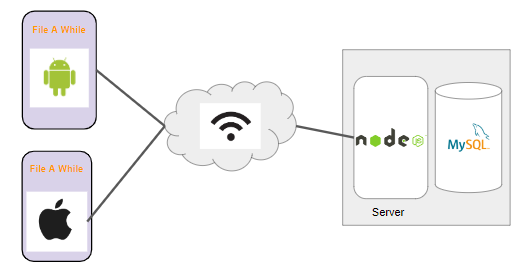
\includegraphics[width=0.7\textwidth]
    {images/Architecture.png}
    \centering
    \label{image:architecture}
    \caption{Architecture}
\end{figure}

\section{Application Design}
The login screens and navigation system screens are two essential parts of the application design. The developer created a set of wireframes to mockup the set of required screens before starting the app development process which enabled careful planning of the system design, which is visually represented in Figure \ref{image:wireframe}. The use of wireframes allows quick development since it makes it easier to comprehend the frontend components that are needed and where they should be placed and how the user navigates between them.
\begin{figure}[h!]
    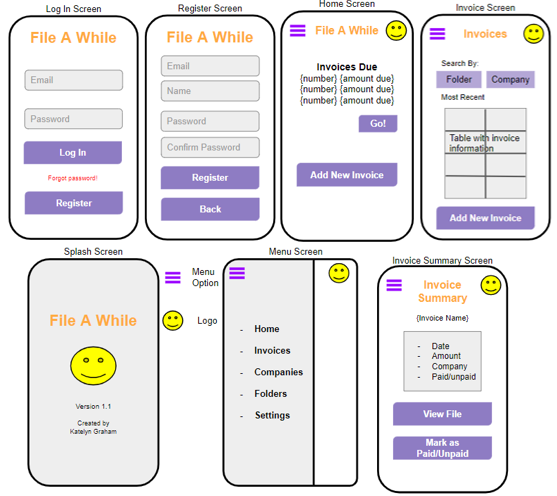
\includegraphics[width=1.0\textwidth]
    {images/AllWireframes.png}
    \centering
    \label{image:wireframe}
    \caption{Wireframes}
\end{figure}

\subsection{Authentication}
The Registration Screen and the Login Screen are two separate screens that make up the authentication screens. The application also includes a splash screen, which is prominently displayed when it is first launched, as seen in Figure \ref{image:splash}. The Splash screen includes a brief display of the application name, creator, and version number along with an image of the app logo, Figure \ref{image:logo}. In order to achieve a smooth transition to the succeeding panels, a standard loader display is used for the entirety of the splash screen.
\begin{figure}[h!]
    
\includegraphics[width=0.3\textwidth]
    {images/SplashScreen.png}
    \centering
    \label{image:splash}
    \caption{Splash Screen}
\end{figure}

\begin{figure}[h!]
    
\includegraphics[width=0.2\textwidth]
    {images/FileLogo.png}
    \centering
    \label{image:logo}
    \caption{App Logo}
\end{figure}

\subsection{Login Screen}
The log-in interface, Figure \ref{image:login}, is straightforward to avoid confusing the user. To access their account, the user only needs to provide their email address and password. If the user does not currently have an account, they can create one by clicking the Register link that appears beneath the login button, which will direct them to the registration page. 
\begin{figure}[h!]
    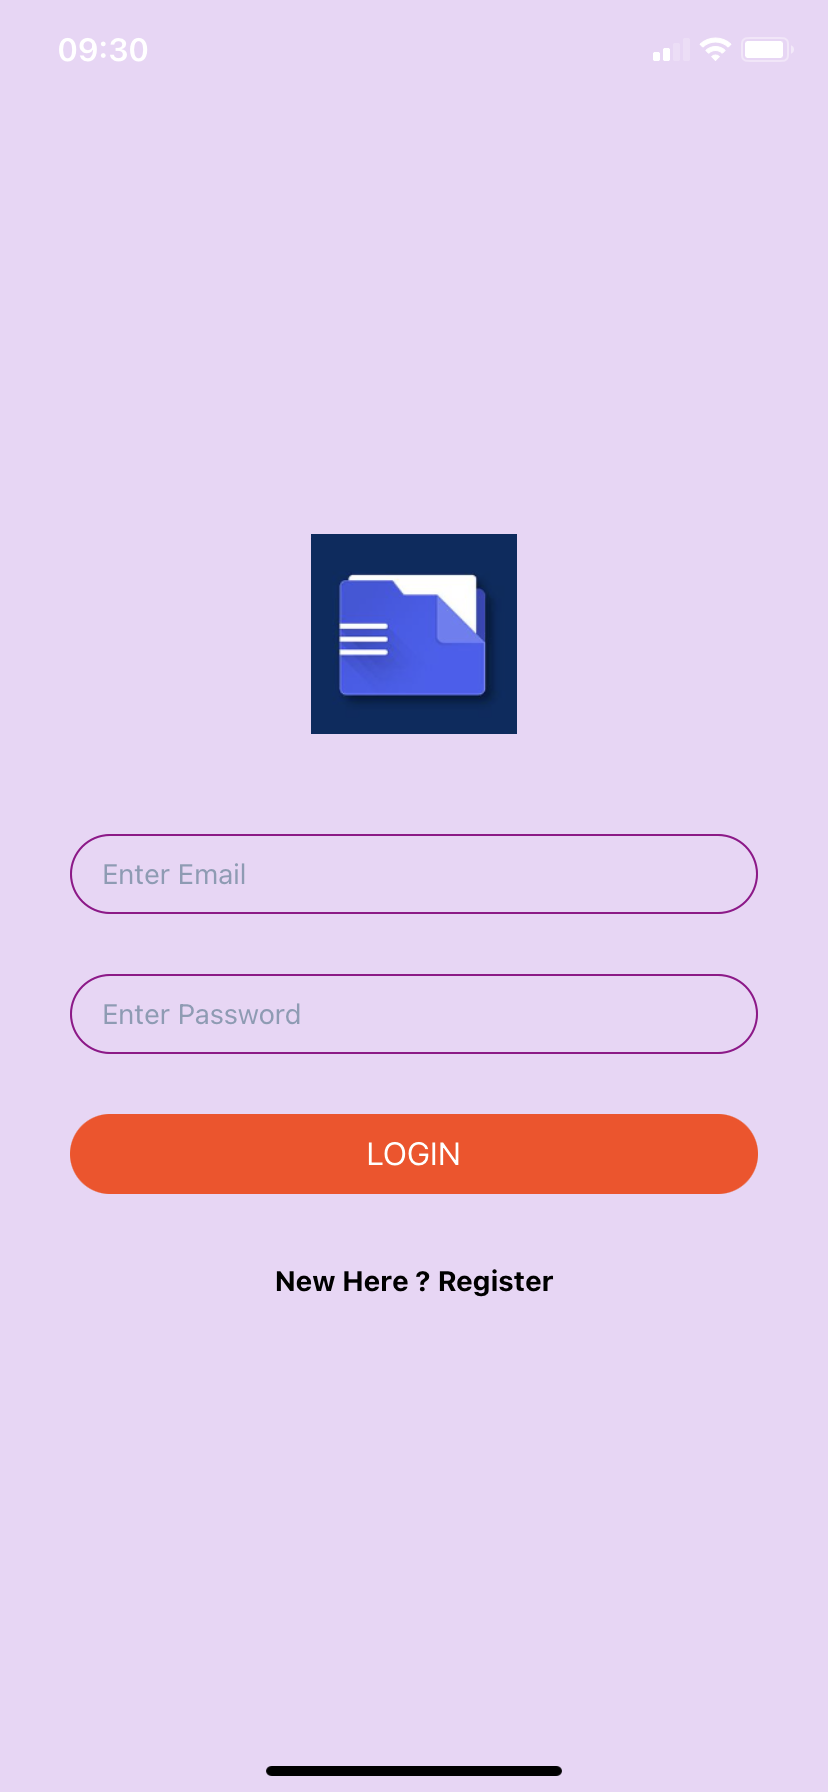
\includegraphics[width=0.3\textwidth]
    {images/Login.png}
    \centering
    \label{image:login}
    \caption{Login Screen}
\end{figure}

\subsection{Registration Screen} 
Figure \ref{image:registeration} shows the Registration Screen, which resembles the Login Screen but also includes a name entry box in addition to the email and password input fields. Users will be taken to the Registration Successful Screen, seen in Figure , after clicking the register button and assuming all required fields have been filled out correctly. They can select a button to enter the Login Screen from this location. An alert box will show if a user fails to complete any of the required registration fields, directing them to take the appropriate corrective action.
\newline \newline
A user will be asked to save their password to their Keychain when signing up for an iPhone. By providing face ID for quick and smooth login authentication, this functionality streamlines and accelerates the login process.
\begin{figure}[h!]
    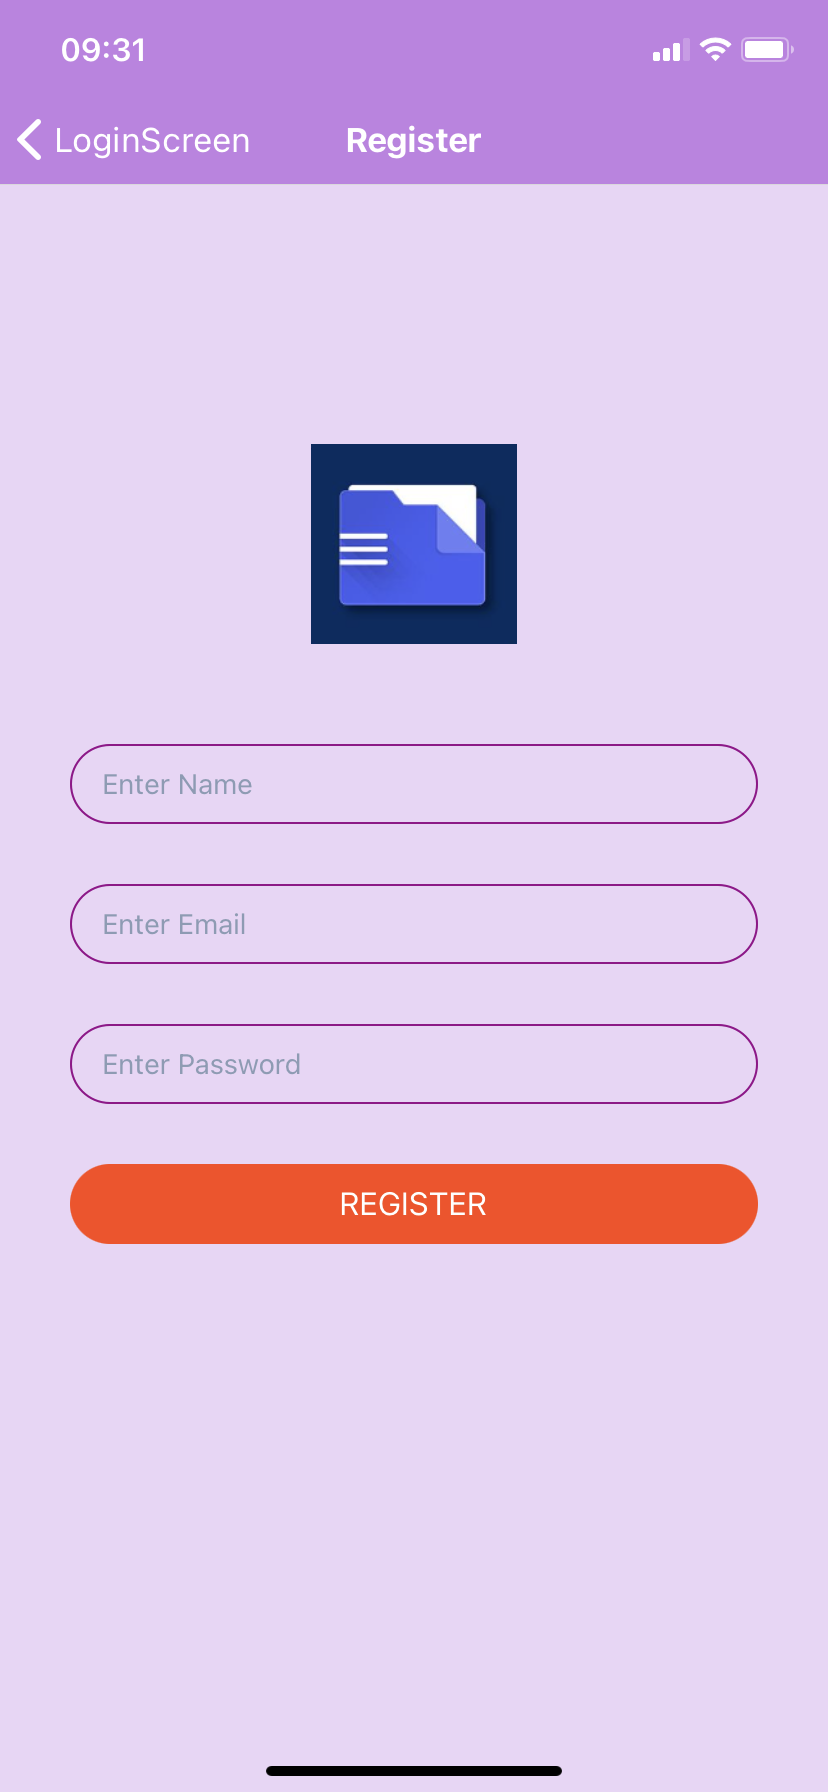
\includegraphics[width=0.3\textwidth]
    {images/Registration.png}
    \centering
    \label{image:registeration}
    \caption{Registration Screen}
\end{figure}
\begin{figure}[h!]
    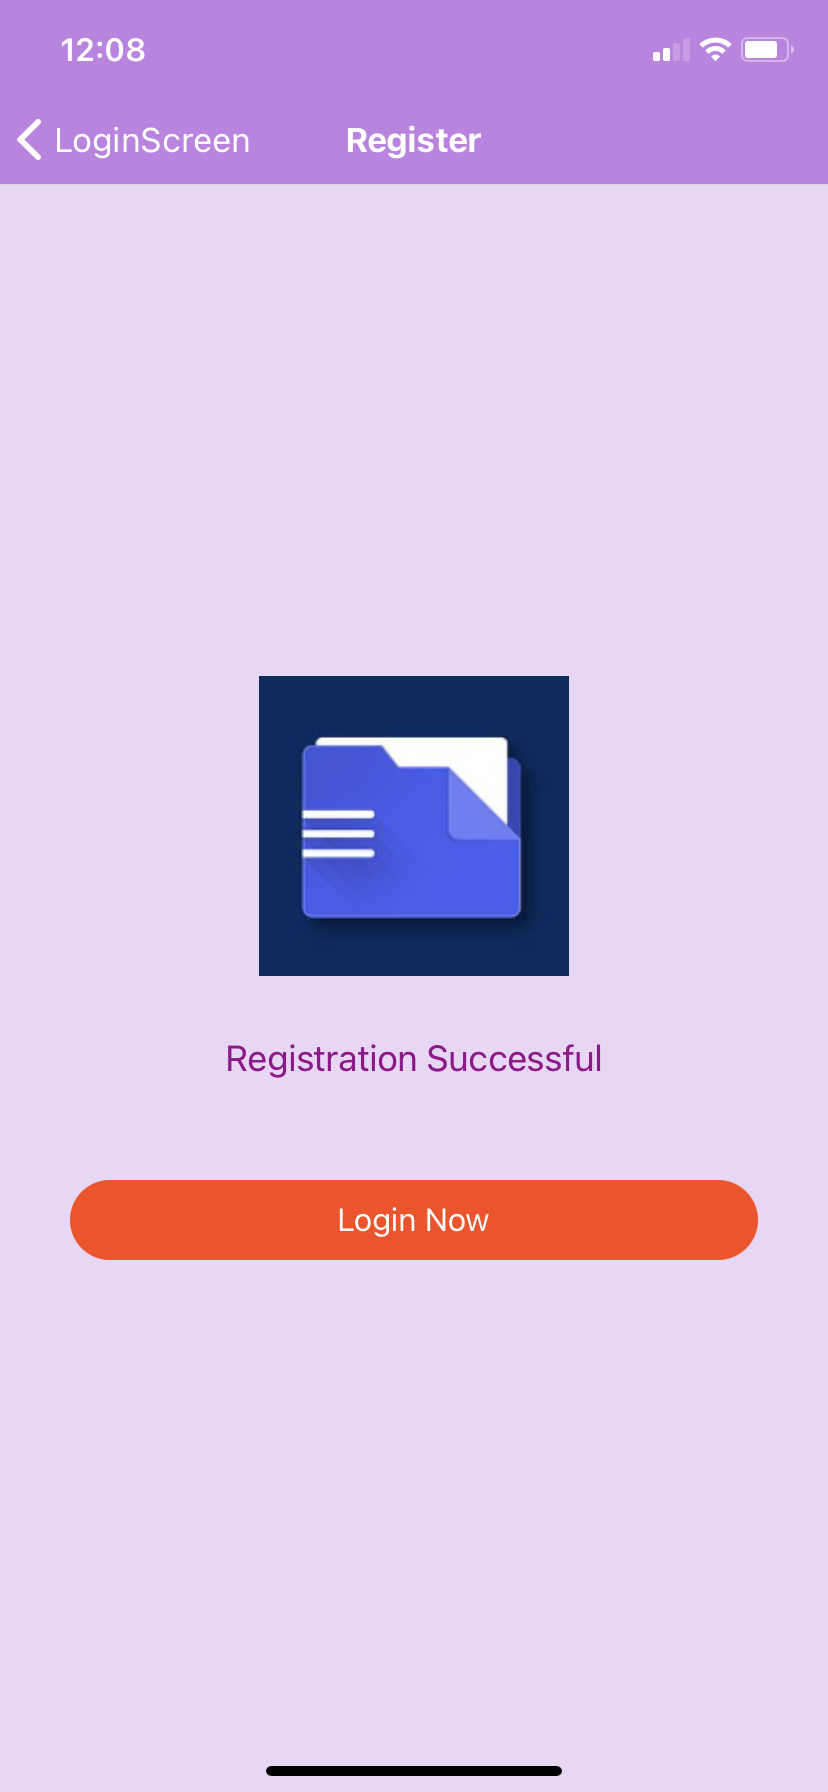
\includegraphics[width=0.2\textwidth]
    {images/RegSuccess.png}
    \centering
    \label{image:regsuccess}
    \caption{Successful Registeration Screen}
\end{figure}

\subsection{Navigation}
The carefully thought-out Drawer Navigation System, shown in Figure \ref{image:nav}, has been created to offer users a handy side menu that can be quickly accessed by swiping from the left edge of the screen or by clicking on the menu symbol located in the upper left corner. The side menu includes a set of options allowing the user to navigate to specific sections of the Application. Users enjoy a simple and efficient navigation process due to the fast presentation of the appropriate screen after selecting a particular item in the menu.
\begin{figure}[h!]
    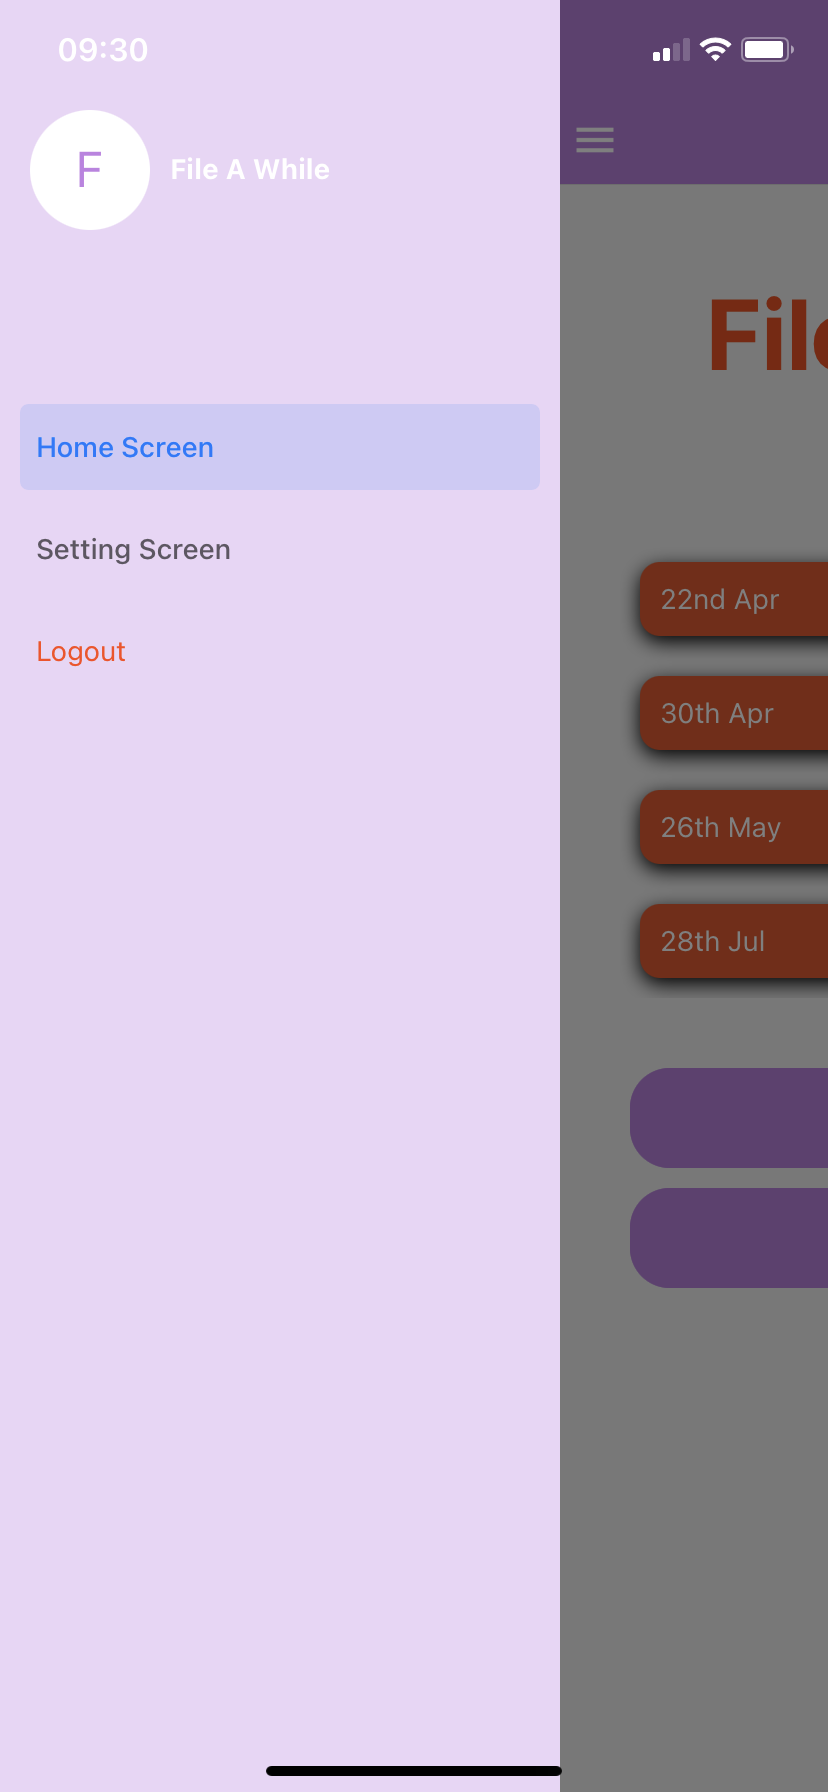
\includegraphics[width=0.3\textwidth]
    {images/Nav.png}
    \centering
    \label{image:nav}
    \caption{Drawer Navigation}
\end{figure}

\subsection{Home Screen}
The Home Screen, \ref{home} which is the user's first screen after logging in, serves as the application's main area. It includes a scrollable list of unpaid invoices, each of which is touchable and, upon selection, takes users to an informative Invoice Summary Page. This page gives a summary of the invoice, including its name, amount, and other important details. Invoices can be marked as paid or completely deleted by users, allowing for effective invoice administration. A back button in the page's upper left corner makes it simple to return to the Home Screen.
\newline \newline
There are two different buttons, each with a different function, underneath the scrollable list. Users who click the first button “Add New Invoice” are taken to a page \ref{allinvoice} that resembles the Home Screen but features a scrollable list that shows every invoice, paid and unpaid. Users can create new invoices on that page by clicking the “Add New Invoice” button. On the Create Invoice screen \ref{create}, the amount and company name of the invoice must be entered, and users can choose a date in the date picker to enter the due date for when the invoice is supposed to be paid. The system will automatically set the due date to the current date if the user forgets to choose one. Additionally, users can change the new invoice's status from unpaid to paid by using the dedicated paid toggle.
\begin{figure}[h!]
    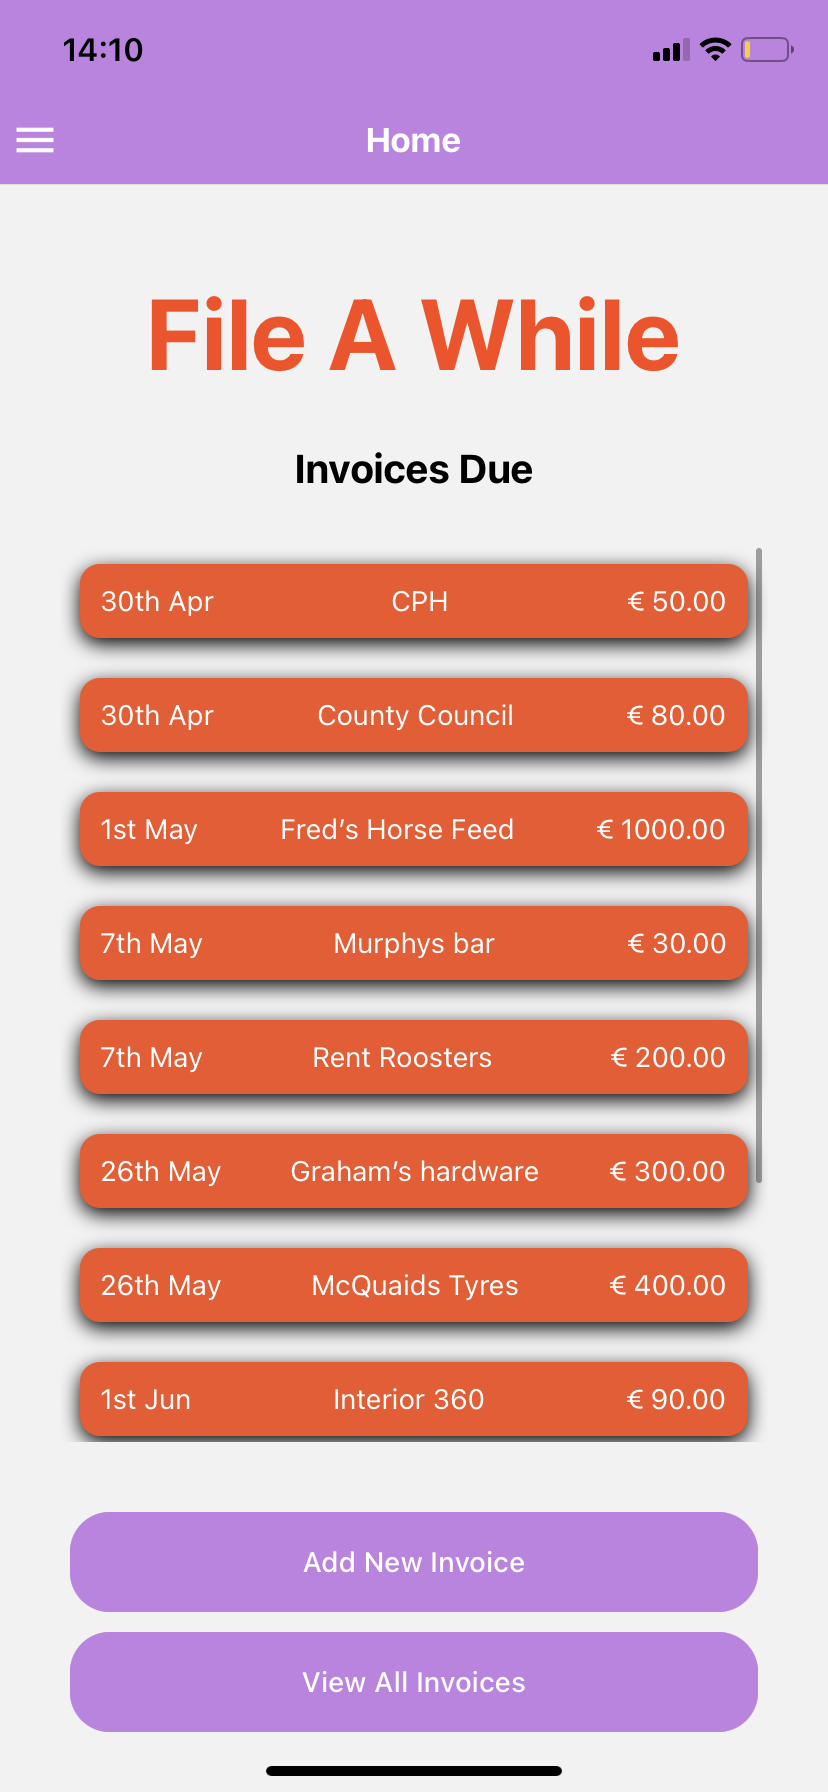
\includegraphics[width=0.3\textwidth]
    {images/Home.png}
    \centering
    \label{image:home}
    \caption{Home Screen}
\end{figure}
\begin{figure}[h!]
    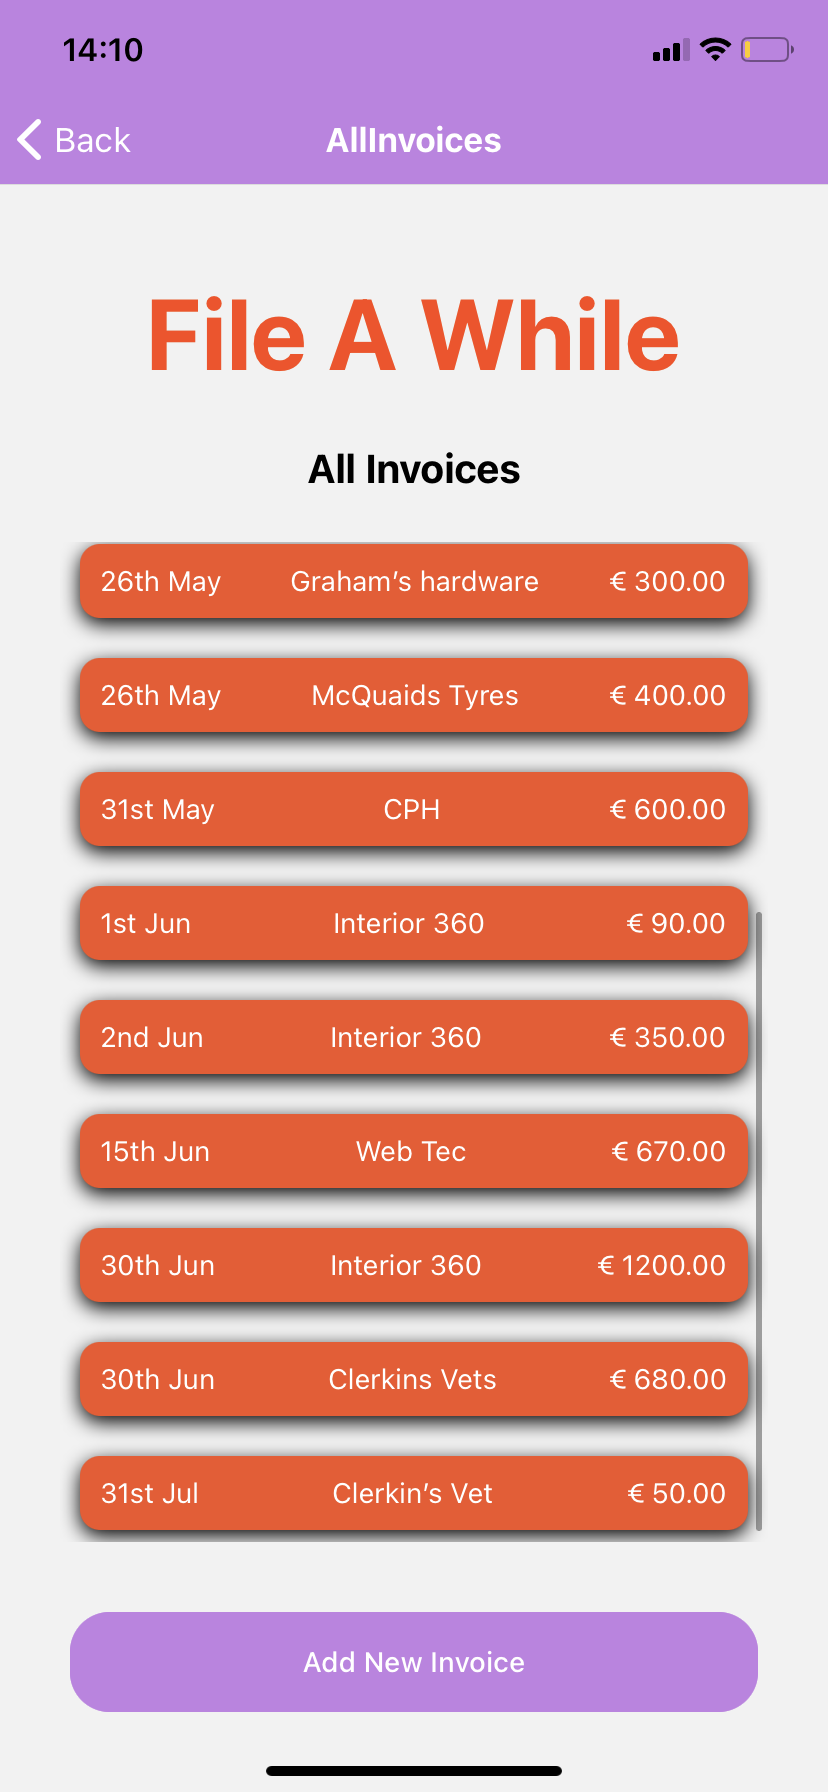
\includegraphics[width=0.25\textwidth]
    {images/AllInvoice.png}
    \centering
    \label{image:allinvoice}
    \caption{All Invoices Screen}
\end{figure}
\begin{figure}[h!]
    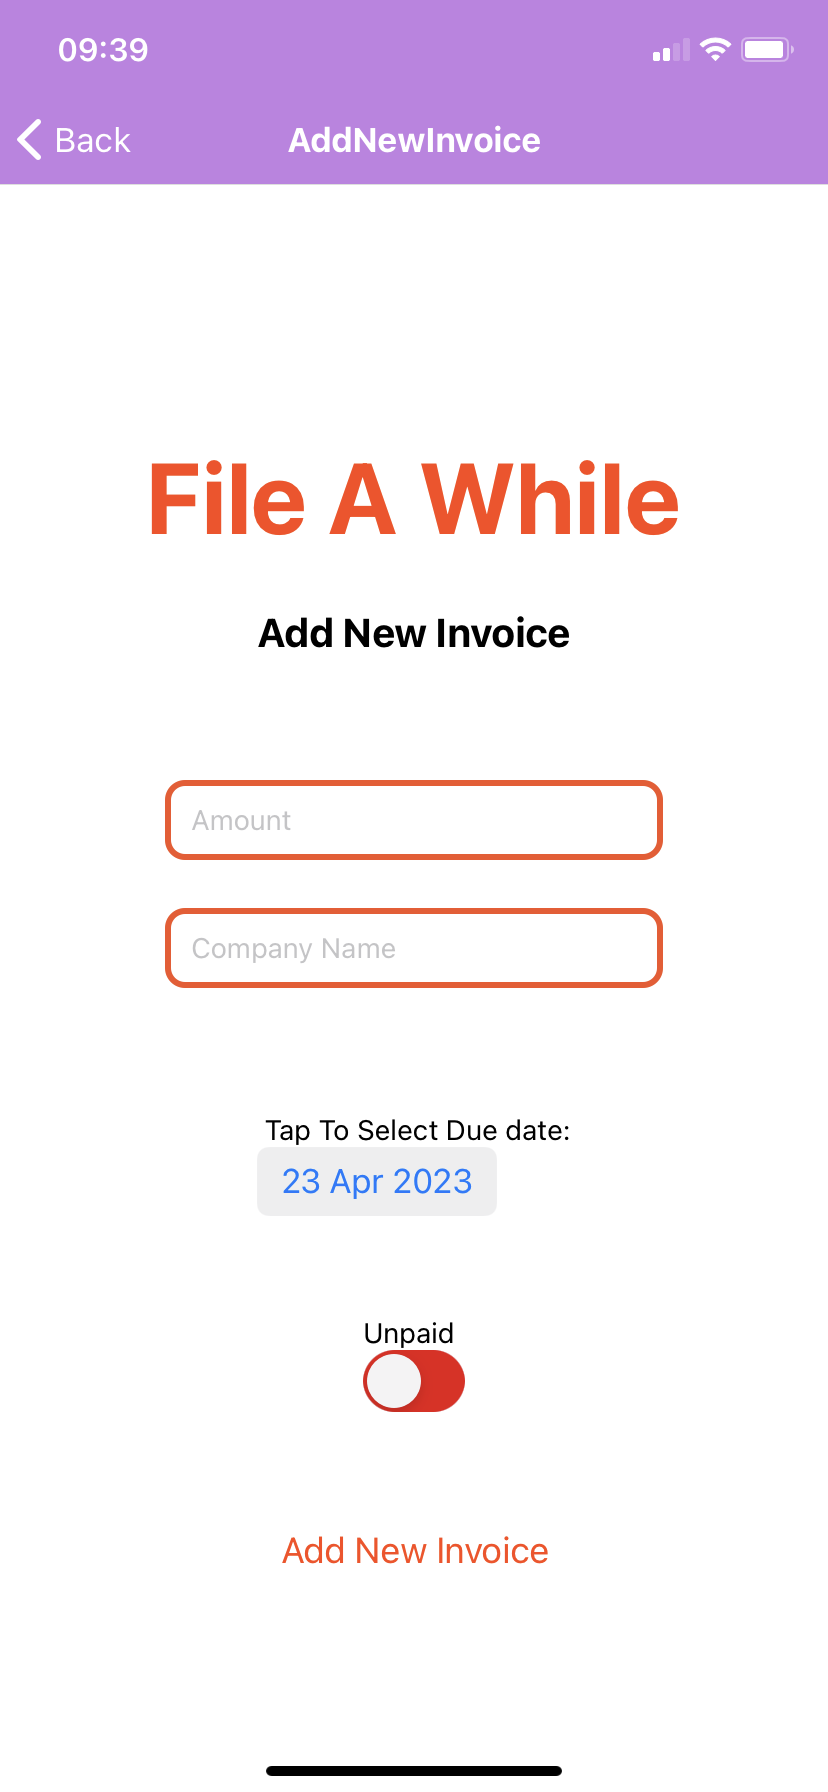
\includegraphics[width=0.25\textwidth]
    {images/Adding.png}
    \centering
    \label{image:create}
    \caption{Add New Invoice Screen}
\end{figure}

\subsection{Settings Screen}
The Settings Screen \ref{setting}, which can be accessed through the Drawer Navigation, gives users the ability to change their account password. Users must be aware of their current password in order to make this change, and they must type in the new password twice while making sure it matches the confirmed password input area. An error message is prominently shown on the screen if users forget their password or enter it incorrectly. It's important to remember that passwords must include a minimum of six characters.
\begin{figure}[h!]
    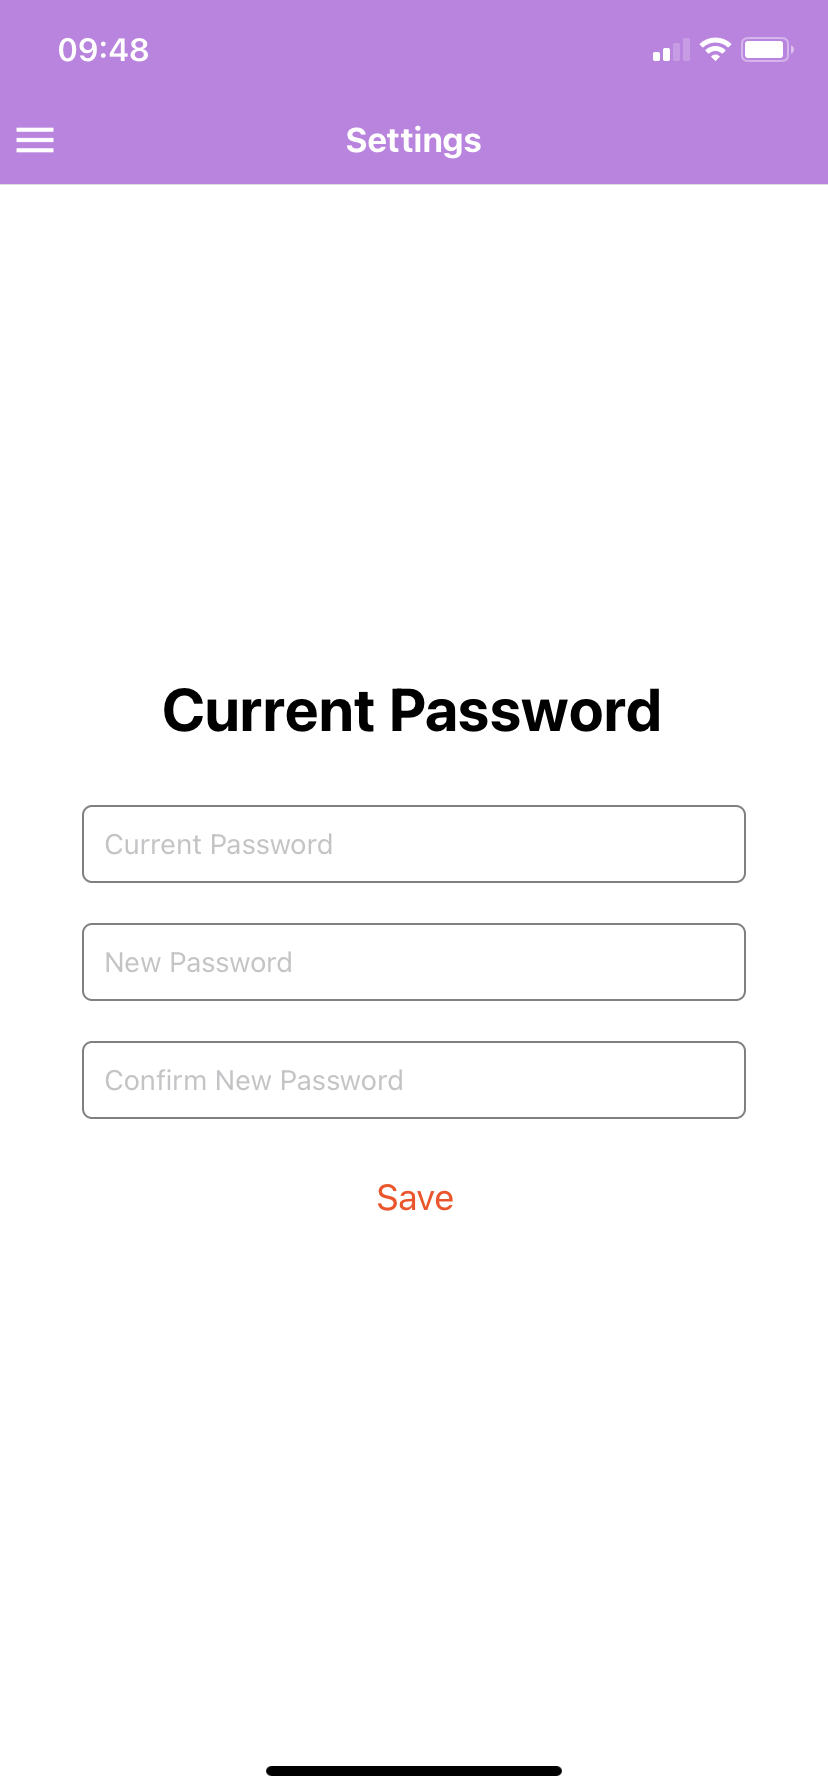
\includegraphics[width=0.3\textwidth]
    {images/Setting.png}
    \centering
    \label{image:setting}
    \caption{Settings Screen}
\end{figure}


\chapter{System Evaluation}

\section{Planning}
At the start of the project, the developer used Jira sprints less strictly than is typical. This strategy caused several issues with work management and progress monitoring, which delayed project completion. After the Christmas break, the developer made the decision to strictly follow the sprint approach, which led to a superior outcome.
It was decided that two-week intervals would be the best size for dividing the sprints. This time frame created a balance between the shortness of a one-week sprint, which might not offer enough time for significant development, and the heavy workload of a sprint lasting longer than two weeks, which might be challenging for the developer to complete in its entirety.
The developer broke down the epics into a number of sub-components, including authentication, dissertation, frontend, backend, and planning, to help with project management. Figure \ref{image:workbreakdown} illustrates how these portions are divided. This divide made it simpler to assign work to team members and monitor progress by helping to identify individual tasks inside each epic.
\begin{figure}[h!]
    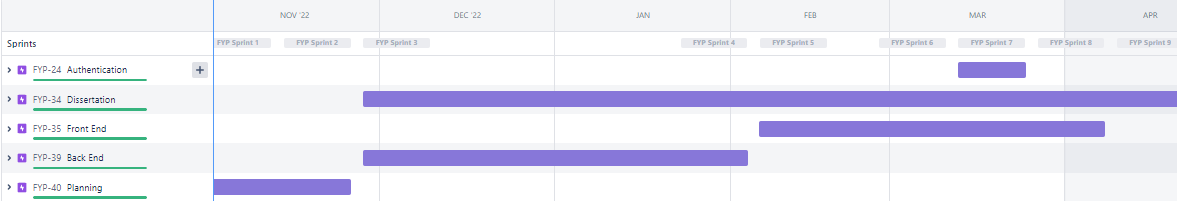
\includegraphics[width=1.0\textwidth]{images/JiraWorkBreakdown.png}
    \centering
    \label{image:workbreakdown}
    \caption{Jira Work Breakdown}
\end{figure}


\section{Testing}
By using Postman to test the backend, the developer was able to properly test the backend functioning, making it simpler to find and fix problems before moving on to the frontend work. This strategy assisted in making sure the backend code was dependable and consistent, which in turn enhanced the application's overall speed.
\newline \newline
The system's backend was tested using Postman, which worked well. The developer was able to manage requests and responses with ease and test the API's different functionalities. In addition, Postman provided a user-friendly interface that made it simple for the developer to write “Automated Tests” to validate the data returned for each of the different API requests. Postmans automated test framework was a big benefit especially as changes were being made to the backend, it was very easy to rerun the automated test suite in postman to make sure that nothing had been broken and if necessary making it simpler to spot any problems and immediately implement fixes.
\newline \newline
Overall, using Postman to test the system's backend was a useful strategy during the application development process. Before beginning frontend development, it enabled the developer to extensively test the backend code and guarantee the overall quality and dependability of the system. The system became stronger and functioned better as a result, which eventually benefited the end users.
\newline \newline


\section{Application}
The method for filing invoices was tested by the developer, who discovered that it worked well overall. The solution seemed to be relevant for small businesses that needed to track their payment and invoicing processes.
\newline \newline
However, upon closer examination, the developer found that they did not make full use of the folder and company backend components. In retrospect, the developer recommendations for future development to include a dropdown list with all potential company names as possibilities in the name input box when submitting a new invoice. A simpler and more efficient invoices procedure would be possible as a result.
\newline \newline
Additionally, the developer recommends creating a company screen where users can view all companies and select them to see all related invoices. This would provide a more organised and user-friendly approach to managing invoicing and payments for multiple companies.
\newline \newline
From a usability point of view it might be beneficial to have a summary / dashboard like screen which showed high level information/ metrics such as the following:
\begin{itemize}
    \item Total Money Due Overall
    \item Total Money Due in Next 7 Days - and if applicable, a button that the user can click to go directly to that specific list of invoices.
    \item Total Money Overdue - with a button that the user can click to go directly to the list of overdue invoices and take action on them
\end{itemize}


\section{Objectives}
The initial objectives of this project was to design and develop an application that facilitated effortless storage of invoices for the end users by offering a user-friendly interface. The project would offer suggestions for improvement in various sections of the application.

\subsection{Were the objectives met?}
Given the limitations of the developer's ability, time, and effort, the project's objectives were successfully met to the greatest extent possible. Despite this, there are still certain things that could be done better, like improving the application's quality. It is stated that the developer's current resources and capabilities place a cap on these advancements. However, the goals that were reached meet the essential requirements and provide a solid groundwork for future progress.

\subsection{Where the objectives were met}

\begin{itemize}
    \item The application successfully eliminates the need for excessive paper documentation and simplifies the process of tracking invoices
    \item The developer learnt how to use React Native effectively and now feels confident to apply it in future application development.
    \item The developer increased their knowledge of JavaScript programming language
\end{itemize}



\chapter{Conclusion} 

The main objective of the current project was to design and build an application that would make it simple for end users to store and manage invoices. The goal of the developer was to create a simple interface for users that would do away with the requirement for extensive paper documentation and simplify the tracking of invoices. The project also provided the developer with the chance to strengthen their programming skills in JavaScript and React Native, which would be extremely helpful in the future when developing new applications. 
\newline \newline
In hindsight, the project has, to a considerable part, succeeded in achieving its goals. The created application efficiently streamlines the handling and storage of invoices while offering users a user-friendly substitute for the challenging paper-based invoice tracking system. The user interface has been thoughtfully created with a focus on usability and effective navigation, eventually improving the user experience. Additionally, the developer has effectively gained proficiency in JavaScript/ NodeJS and React Native development, which can be used in future projects.
\newline \newline
The chapter on system evaluation provided insightful information about the planning, testing, and general application design. The developer initially had trouble following the sprint approach during the planning stage, which caused problems with task management and progress monitoring. The developer decided to carefully adhere to the sprint technique following the holiday break, which resulted in a more efficient and well-organised development process. The two-week sprint intervals turned out to be the best option because they balanced the effort and allowed for enough time to make significant growth progress.
\newline \newline
In terms of testing, the developer used Postman to carefully review the application's backend functioning. This approach made it possible to find problems early on and fix them, guaranteeing the consistency and dependability of the backend code. As a result, the application's overall performance improved, which benefited the end users. An efficient analysis of test results was made possible by Postman's user-friendly interface, which made it a useful tool for backend testing.
\newline \newline
A close examination of the application's design revealed that the mechanism for filing invoices generally functioned well and was deemed appropriate for small businesses needing a solution for monitoring the payment and invoicing processes. The developer admitted that the folder and company backend components' full potential had not yet been achieved. As a result, the developer advised adding a dropdown list with alternatives for company names to the name input box when producing a new invoice. The process of invoicing would be simplified, and efficiency would improve. The developer also proposed making a panel for companies so users could examine all firms and pick them to view the bills that go with them. With this improvement, managing invoicing and payments for various businesses would be easier to manage, both in terms of organisation and usability.
\newline \newline
In summary, the project has been successful in achieving its core objectives of developing an invoice management application that is both user-friendly and efficient. The application provides users with an easy-to-use solution and tackles the main problems associated with traditional paper-based invoice tracking solutions. 
\newline \newline
In conclusion, the created application provides a strong base for further growth and development. The programme can develop into a more complete and reliable solution for invoice management by adding new features, improving user experience, and improving the performance and security. There is tremendous potential for the programme to develop into an essential tool for companies and individuals looking for a cutting-edge and effective method of managing their invoices as long as the developer keeps building upon what has been achieved and lessons learnt from this project.

\appendix
\chapter{Git Hub Links}

\section{Applied Project}

The below URL directs to the primary Git repository used for this project’s development. It contains all the code from the frontend and backend.

\href{https://github.com/katelyngraham1/Final_Year_Project}{https://github.com/katelyngraham1/Final\textunderscore Year\textunderscore Project} 


\section{Dissertation} 
This URL points to the source control for this latex document. Readers can refer to the above repository for more detail on the project’s implementation.

\href{https://github.com/katelyngraham1/Final_Year_Dissertation}
{https://github.com/katelyngraham1/Final\textunderscore Year\textunderscore Dissertation}



\section{Video Demo}
This URL points to the demo video. This video goes through the application and explains how to use the it.

\href{https://youtu.be/oJY_FlK4dSM}
{https://www.youtube.com/watch?v=oJY\textunderscore FlK4dSM}




%------------------------------------------------------------------------------------------------------	
% Generate the bibliography. You may have to build the document more than once before all of the
% references and processed and cited correctly.
% WARNING: Don't mess with any of the following unless you know what you are doing.
%------------------------------------------------------------------------------------------------------	
\bibliographystyle{unsrt}
\bibliography{references.bib}
\end{document}
